\documentclass[11pt,letterpaper]{article}
%\documentclass[11pt,a4paper]{report}

\usepackage{amssymb,amsmath,amsthm} 
\usepackage[margin=2cm]{geometry}
\usepackage{fancyhdr}
\usepackage{enumitem}
\usepackage[compact]{titlesec}
\usepackage{graphicx,ctable,booktabs,subcaption}

\usepackage{blkarray}

\usepackage{xparse,hyperref,parskip}

%\newcommand{\abs}[1]{\left|#1\right|}

\newcommand{\semester}{Spring 2022}
\newcommand{\due}{Tuesday, March 22}

\newcommand{\bigo}{\mathcal{O}}

\pagestyle{fancy}
\lhead{ }
\chead{\footnotesize Math 3338\quad  Numerical Methods\quad  \semester}
\rhead{\footnotesize \thepage}
\setlength{\parindent}{0cm}
\setlist{noitemsep}



\newtheorem{theorem}{Theorem}

\input{defs.tex}

%Defines the problem environment with arguments Points and Solution gap
\input{problem_env.tex}



\begin{document}

\begin{center}
{\huge{\bf  Numerical Methods}} \\[1.5ex]
{\bf Math 3338 -- \semester}\\[1.5ex]
{\Large{\bf Worksheet 17\ \\[2ex] Eigenvector Applications - Markov Chains}}\\
\end{center}
\vspace{2mm}



\section{Reading}

\begin{table}[!ht]
 \centering
 \begin{tabular}{ll}
   CP &   \\
 NMEP &  
 \end{tabular}
\caption{Sections Covered}
\end{table}


\section{What is a Markov Chain}
Think about a system with a sequence of states $s_n$ so that the probability of $s_n$ depends only on $s_{n-1}$. A classic example is a simple board game like Chutes and Ladders, where you land at the end of the turn depends only on where you are now. 

Let's do an example. Figure \ref{fig:simple_game} shows a very simple game. 
\begin{figure}[!h]
 \centering
 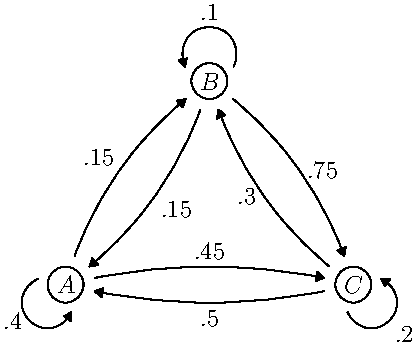
\includegraphics{images/simple_game.pdf}
 \caption{A simple game.}
 \label{fig:simple_game}
\end{figure}
If you are standing on $A$, you have a .15 probability of moving to $B$, .45 of moving to $C$ and a .4 of not moving at all. Using this we can create a matrix.
\begin{equation}
M  = 
\begin{blockarray}{cccc}
 & \color{gray}{A} & \color{gray}{B} & \color{gray}{C} \\
\begin{block}{c[ccc]}
  \color{gray}{A} & .4 & .15  & .45 \\
  \color{gray}{B} & .15 & .1  & .75 \\
  \color{gray}{C} & .5 & .3 & .2 \\
\end{block}
\end{blockarray}
\end{equation}
The matrix $M$ is the transition matrix of Figure \ref{fig:simple_game}. Notice the sum of each row is 1, this should tell you have the matrix is arranged. 

Let our sequence of states be denoted by $x_n$ and say we start on $A$, then $x_0 = \begin{bmatrix} 1 \\ 0 \\ 0\end{bmatrix}$. We want to know the probability of being on each vertex after 1 `round'. We should be able to use logic to determine\footnote{If this isn't clear, think about the probability of going to each space starting on $A$.} that $x_1 = \begin{bmatrix} .4 \\ .15 \\ .45 \end{bmatrix}$. Of course, to find $x_2$ it becomes much more difficult. This is where the Markov matrix becomes useful, notice $x_1 = Ax_0$. Expanding on this we see,
\begin{align*}
 x_n = & Ax_{n-1} \\
  = & AAx_{n-2} \\
  = & A^2x_{n-2} \\
  = & \dots \\
  = & A^n x_0
\end{align*}
If we let $x=\lim x_n$ then $x = Ax$, which implies that $x$ is an eigenvector of $A$ and $1$ is an eigenvalue\footnote{Assuming that the sequence converges, which it turns out always does for Markov matrices.}. This is actually a little hand wavy at the moment. In reality, we want to find $A^n$. Think about diagonalizing $A$, 
\[
P^{-1}AP = D
\]
Recall from linear algebra that $P$ is the matrix of eigenvectors of $A$ and $D$ is the diagonal matrix with eigenvalues on the diagonal. Then $A^n = (PDP^{-1})^n = P D^n P^{-1}$. The eigenvalues of a markov matrix all satisfy $\abs{\lambda}\le 1$ with exactly one equal to 1. This implies $D^n$ converges to a matrix with exactly one 1 on the diagonal and 0's everywhere else. 

The steady state matrix $A_{steady} = P \begin{bmatrix} 1 & 0 & \dots & 0 \\ 0 & 0 & \dots & 0 \\ \vdots & \vdots &\ddots &\vdots \end{bmatrix}P^{-1}$ is the ultimate convergence of the system. In otherwords, if you played an infinite number of rounds, the entries of $A_{steady}$ would be the probability you'd be on any space given a starting point. 



\newpage

\begin{center}
{\huge{\bf  Numerical Methods}} \\[1.5ex]
{\bf Math 3338 -- \semester}\\[1.5ex]
{\Large{\bf Homework 17 (Due: \due)}}\\
\end{center}
\vspace{2mm}

\begin{problem}
 Create a function \texttt{steady\_state(A)} that returns the steady state of a Markov matrix $A$. You can always test your answer by choosing a matrix $A$ and taking repeated powers; however, your function should be smarter than that. 
\end{problem}


For Problems \ref{simple-start} -- \ref{simple-end} use the board in Figure \ref{fig:simple_game}.

\begin{problem}
 \label{simple-start}
 If you start on $A$, what is the probability you land on $A$ again after
 \begin{enumerate}
  \item 1 round
  \item 10 rounds
  \item 100 rounds
  \item 1000 rounds
 \end{enumerate}
\end{problem}

\begin{problem}
 Find the steady state of the board. What is the probability you are on $A$ in the steady state if you start on $A$?
\end{problem}


\begin{problem}
 \label{simple-end}
 This is an optional, but highly recommended, problem. Create a simulation that will play \texttt{N} rounds on the board starting on $A$. What do I mean? You start on $A$ and the next turn you have a .15 probability of moving to $B$. Do not use a Markov matrix to solve this problem, you want explicit states, not probabilities. Create a function called \texttt{play\_round(B,location)} where \texttt{B} is the board and \texttt{location} is your current location. This will return the next location. Next create a function \texttt{play\_game(B,N)} where $B$ is the board and $N$ is the number of rounds. Use these functions to simulate 1000 games of 100 rounds each. 
 
 Find the distribution of your location after each of the 100 rounds (i.e. add all the states and divide by 1000). Compare this to $A^{100}v$ where $v$ is the vector corresponding to starting on $A$. How close are your answers? 
\end{problem}


\begin{problem}
 Let's play Chutes and Ladders see Figure \ref{fig:chutes} for the board. The way the game works is you spin a dial and move 1, 2 or 3 spaces. If you land at the bottom of a ladder, you go to the connected space. Top of a slide? You're going backwards. For example, if you land on space 3, you advance to space 10. If you land on space 42\footnote{You need to land exactly on the space, so if you roll a 3 on space 40 you stay on space 40.}, you win! 
 
 \begin{enumerate}
  \item Create the Markov matrix for this board. This will be a large, sparse matrix. Try to be clever about how you represent it and enter it into Python (you'll eventually want to turn it into a numpy matrix).
  \item How many rounds do you need to play before the probability of winning is greater than 50\%?
  \item What does the steady state matrix look like for this game? Explain why.
  \item Create a function \texttt{heatmap(B,n)} that creates a heatmap of likely locations in round n. The function \texttt{matplotlib.pyplot.imshow} will probably be useful as will reshaping arrays using numpy.
 \end{enumerate}
 
 \begin{figure}[!h]
  \centering
  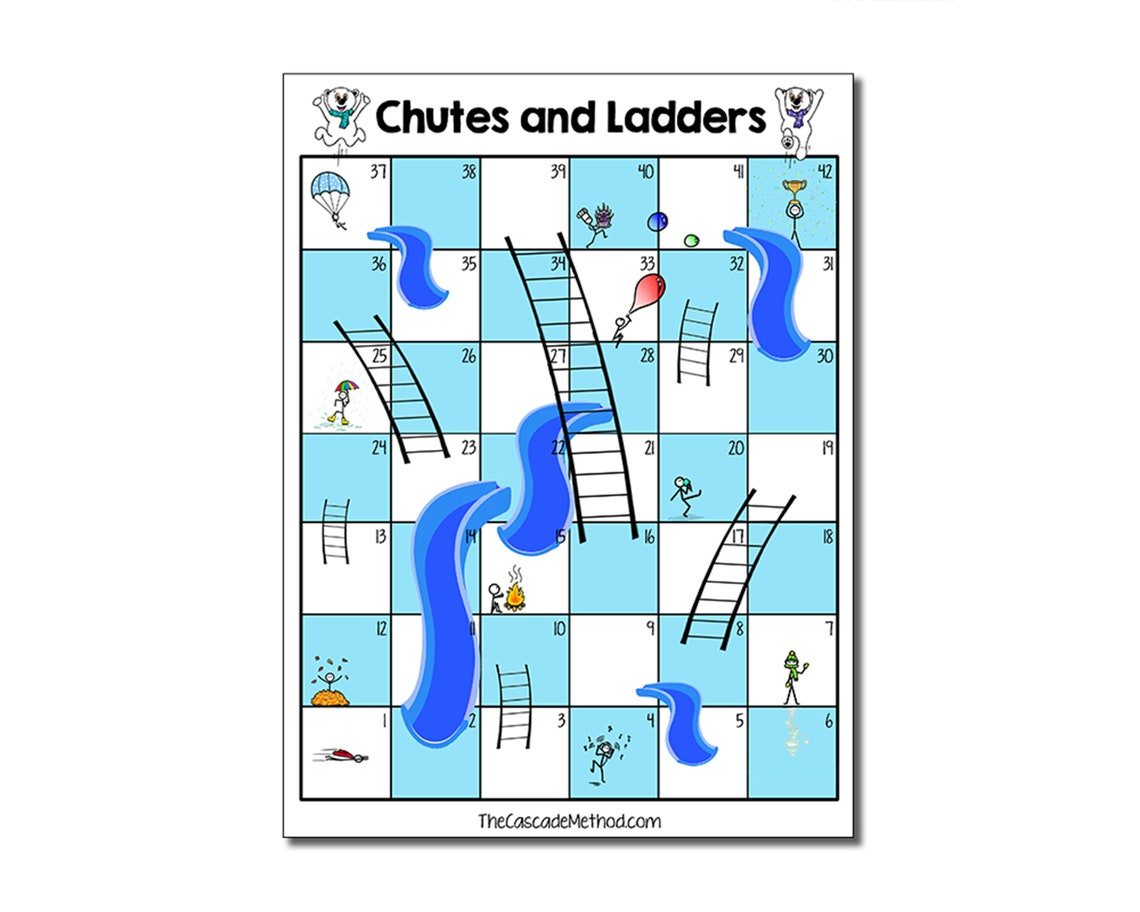
\includegraphics[width=1\textwidth]{images/chutes.jpg}
  \caption{Chutes and Ladders}
  \label{fig:chutes}
 \end{figure}
\end{problem}


\end{document}





































